\subsection{Software Development Process}
\label{subsec:soft_dev}
Because of the expected tight time constraints during system 
development, the author of this paper chose an Agile Software 
Development Methodology. Agile Sprints were primarily used to manage 
time efficiently during the software development process
\cite{JavaTPointAgile, Milne2021}. Moreover, a modified Agile Development Methodology as
shown in Figure \ref{fig:agile} was followed in the system
development procedures for this special problem.

% Agile Development
\begin{figure}[ht]
    \centering
    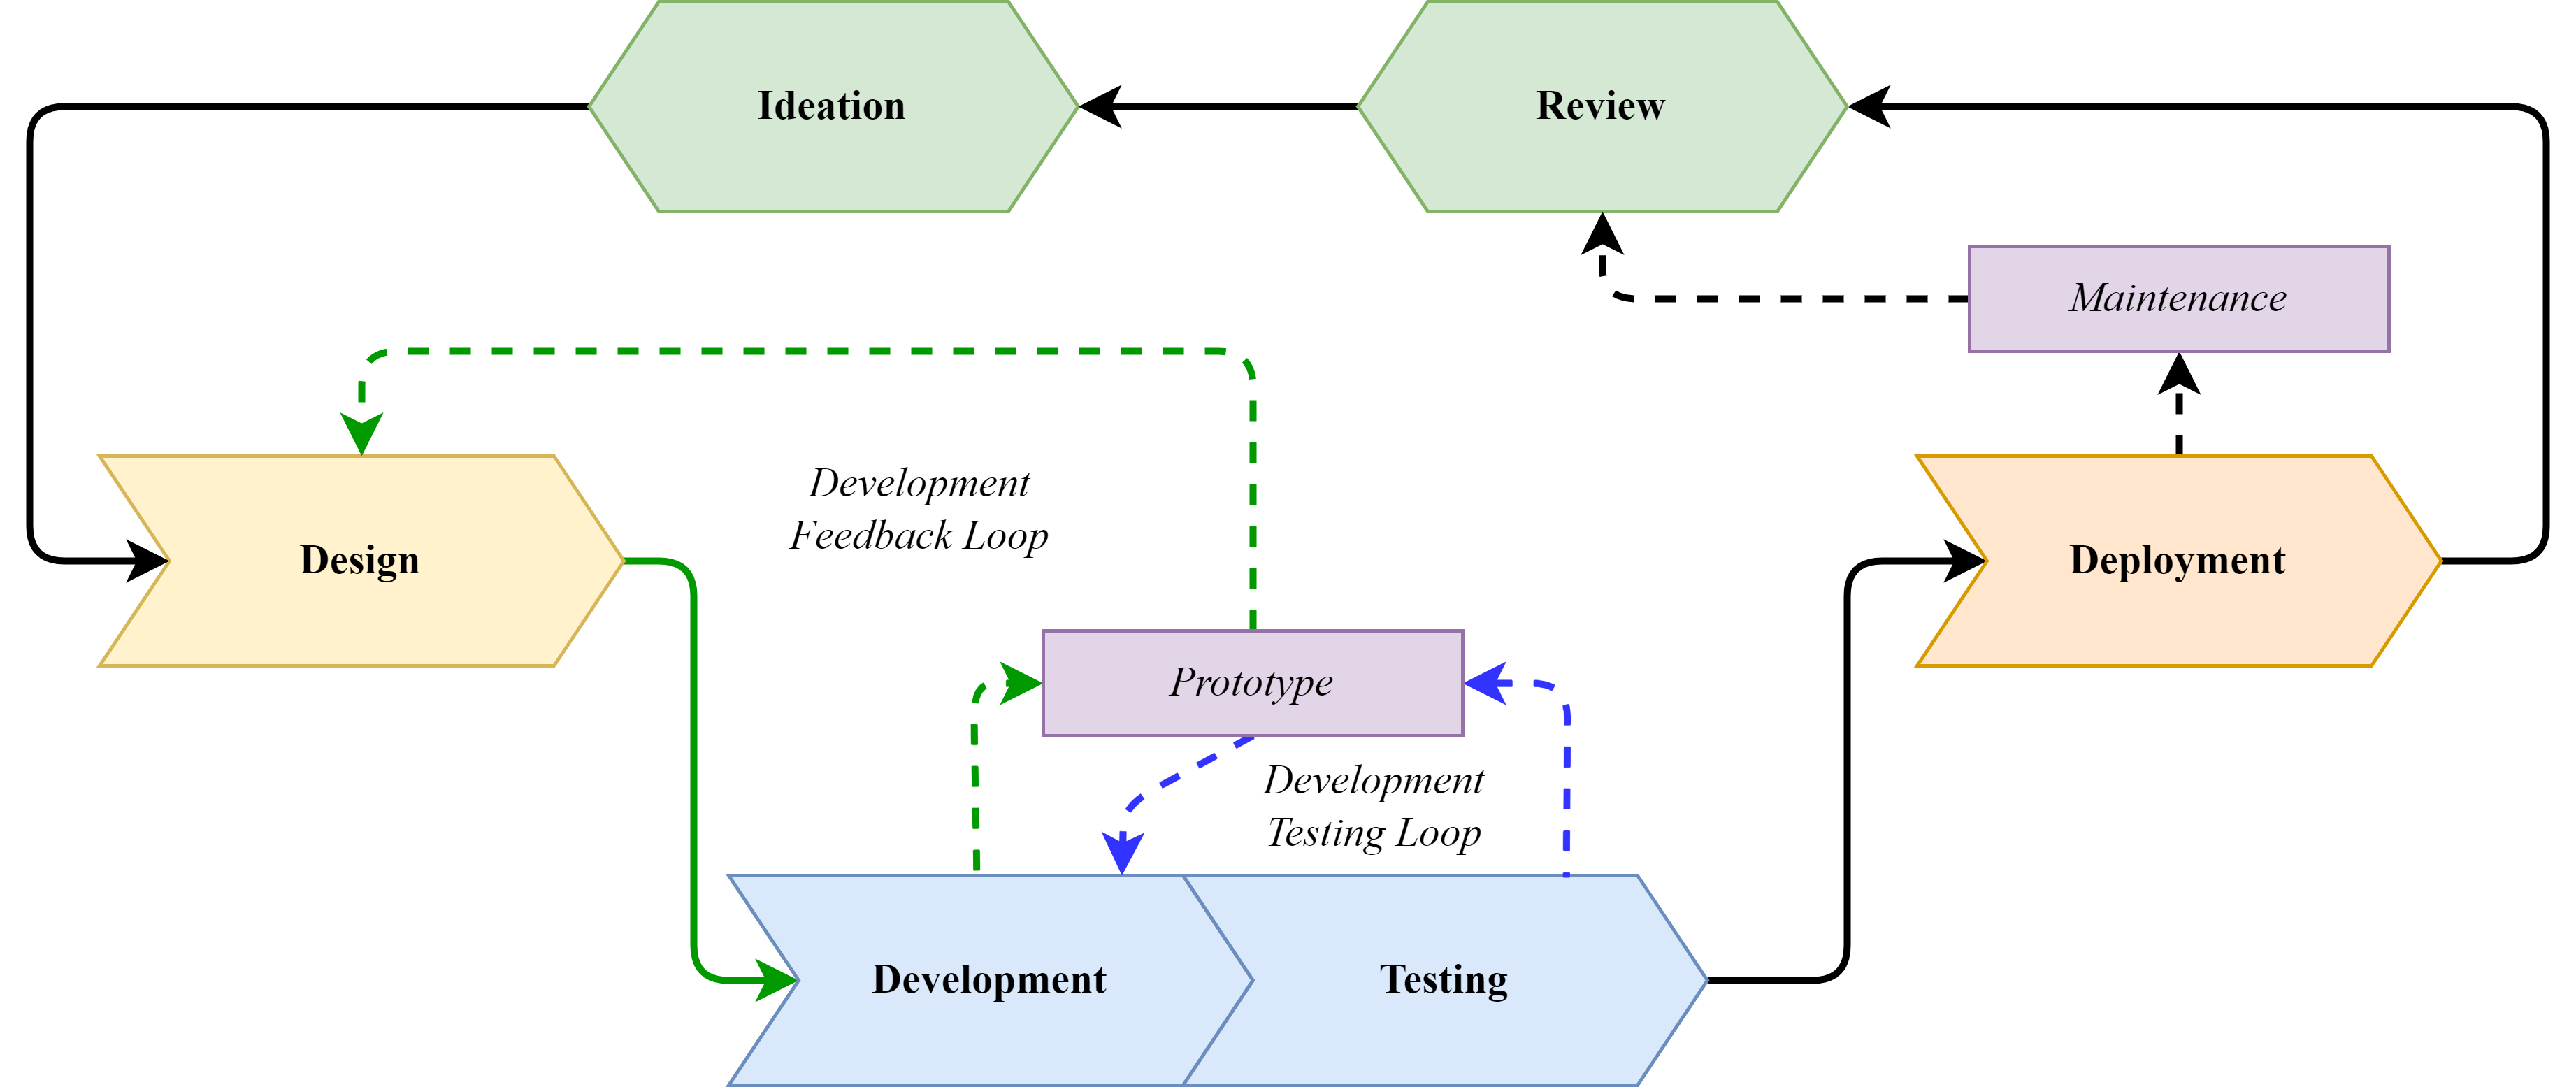
\includegraphics[width=1\textwidth]{./assets/Chapter_3/agile.png}
    \caption{Modified Agile Development Methodology}
    \label{fig:agile}
\end{figure}
\FloatBarrier

The modified agile development methodology shown above includes 
additional and specific "feedback loops" such as a development 
feedback loop that focuses on the continuous design and development 
process; and a development testing loop that ensures that the 
software being developed works as intended or better than expected.
\hfill \\

The Table \ref{summary-sprints} shows the list of sprints and 
sub-activities that were followed:
\hfill \\

% TABLE: SPRINTS AND SUB-ACTIVITIES
\begin{longtable}{|c|l|l|}
    \caption{Summary of Sprints and Activities}
    \label{summary-sprints}\\
    \hline
    % Header
    \textbf{Sprint Number} & 
    \multicolumn{1}{c|}{\textbf{Activities}} & 
    \multicolumn{1}{c|}{\textbf{Completion Date}} \\ \hline
    \endfirsthead
    % Continued Header
    \multicolumn{3}{c}%
    {{\bfseries Table \thetable\ continued from previous page}} \\
    \hline
    \textbf{Sprint Number} & 
    \multicolumn{1}{c|}{\textbf{Activities}} & 
    \multicolumn{1}{c|}{\textbf{Completion Date}}\\ \hline
    \endhead
    % Row 1
    1 &
    \begin{tabular}{p{0.35\textwidth}}
        \textbf{Main Activity:} Requirement Analysis, System Planning, and Evaluation\\
        \vspace{0.5cm}
        \textbf{Sub-Activities:}
        \begin{itemize}
            \item Topic Proposal 
            \item Drafted Chapters 1 to 3 for the Special Problem Proposal
            \item System Architecture and User Requirement Analysis
        \end{itemize}
    \end{tabular} &
    \begin{tabular}{p{0.20\textwidth}}
        September 15, 2022 to December 9, 2022
    \end{tabular} \\ \hline
    % Row 2
    2 &
    \begin{tabular}{p{0.35\textwidth}}
        \textbf{Main Activity:} Development of Initiasl Sytem Prototype\\
        \vspace{0.5cm}
        \textbf{Sub-Activities:}
        \begin{itemize}
            \item Build the different component of the alamSYS as 
            indicated in the top-level overview diagram of the system, 
            the following prototype were initially developed:
            \subitem[1.] API endpoints
            \subitem[2.] Database
            \subitem[3.] Preprocessor
            \item Tested the build prototype.
        \end{itemize}
    \end{tabular} &
    \begin{tabular}{p{0.20\textwidth}}
        \textbf{12 Weeks}
        September 30, 2022 to December 23, 2023
    \end{tabular} \\ \hline
    % Row 3
    3 &
    \begin{tabular}{p{0.35\textwidth}}
        \textbf{Main Activity:} Development and Testing of
        DMD-LSTM Model \\
        \vspace{0.5cm}
        \textbf{Sub-Activities:}
        \begin{itemize}
            \item Stock Market Data until February 10, 2023 was
            collected.
            \item Development of the Deep Learning Model. following
            the procedures as previously discussed on section
            \ref{subsec:ml_diagram}.
            \item Development of Baseline LSTM model for comparison
            against DMD-LSTM Model.
            \item Deep Learning model training, testing, cross-validation,
            and evaluation.
            \item Revised of Chapters 1 to 3.
        \end{itemize}
    \end{tabular} &
    \begin{tabular}{p{0.20\textwidth}}
        January 1, 2023 to February 21, 2023
    \end{tabular} \\ \hline
    % Row 4
    4 &
    \begin{tabular}{p{0.35\textwidth}}
        \textbf{Main Activity:} Integration of DMD-LSTM Model 
        to the alamSYS and System Testing\\
        \vspace{0.5cm}
        \textbf{Sub-Activities:}
        \begin{itemize}
            \item Integrated DMD-LSTM to alamSYS.
            \item Initial tests of the system.
            \item Created System Tests and Loggers.
            \item System Testing, Results Logging and Summarization.
        \end{itemize}
    \end{tabular} &
    \begin{tabular}{p{0.20\textwidth}}
        January 15, 2023 to March 7, 2023
    \end{tabular} \\ \hline
    % Row 5
    5 &
    \begin{tabular}{p{0.35\textwidth}}
        \textbf{Main Activity:} System Testing, Analysis, Refactoring, and Deployment\\
        \vspace{0.5cm}
        \textbf{Sub-Activities:}
        \begin{itemize}
            \item Development test loop was conducted.
            \item System  Refactoring.
            \item System Update and inclusion of additionl features.
            \item Results Gathering and Summarization.
            \item Started the development of the test application 
            (for showcasing of the system features).
        \end{itemize}
    \end{tabular} &
    \begin{tabular}{p{0.20\textwidth}}
        March 7, 2023 to April 13, 2023
    \end{tabular} \\ \hline
    % Row 6
    6 &
    \begin{tabular}{p{0.35\textwidth}}
        \textbf{Main Activity:} Finalization of Paper, System Defense, and Presentation\\
        \vspace{0.5cm}
        \textbf{Sub-Activities:}
        \begin{itemize}
            \item Revised Chapter 1 to 3.
            \item Drafted Chapter 4 to 5.
            \item Finalization of the mobile-based test application.
            \item Reviewed the Content of this paper.
            \item Revised and Finalized the special problem paper.
            \item Created presentation slide deck for the presentation 
            of the special problem.
        \end{itemize}
    \end{tabular} &
    \begin{tabular}{p{0.20\textwidth}}
        March 14, 2023 to May 12, 2023
    \end{tabular} \\ \hline
\end{longtable}

From Table \ref{summary-sprints}, it was
shown that it took a total of 34 weeks (from September 15, 2022, 
to May 12, 2023) to develop the alamSYS and all its components, as
well as to write the contents of this paper. This was 5 weeks
better than the expected total weeks allotment for the completion
of this whole project, as projected in the Gantt Charts shown in
Appendix \ref{sec:appendix_b}.